{\color{indiagreen}\subsection{Delo pri raztezanju idealno prožne vzmeti}}
\begin{center}
	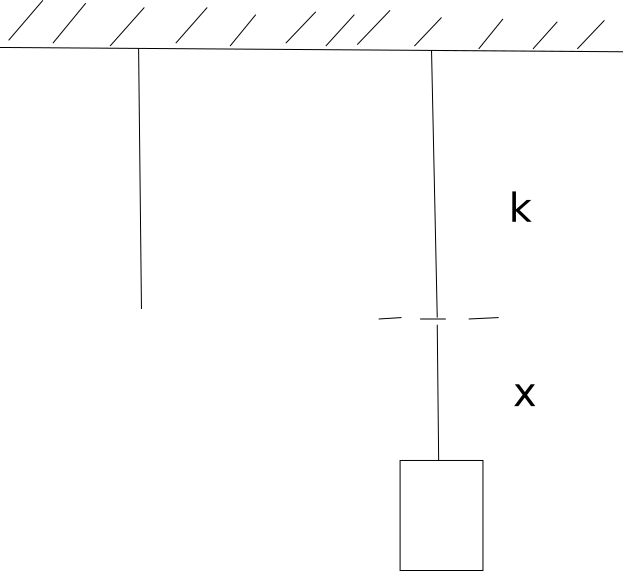
\includegraphics[width=15cm, height=15cm,keepaspectratio=true]{Vzmet.png}
\end{center}
\begin{align*}
	A &= \overline{F}s \leftarrow x\\
	\overline{F} &= \frac{0 + kx}{2} = \frac{kx}{2}\\
	A &= \frac{kx^2}{2}\\
\end{align*}
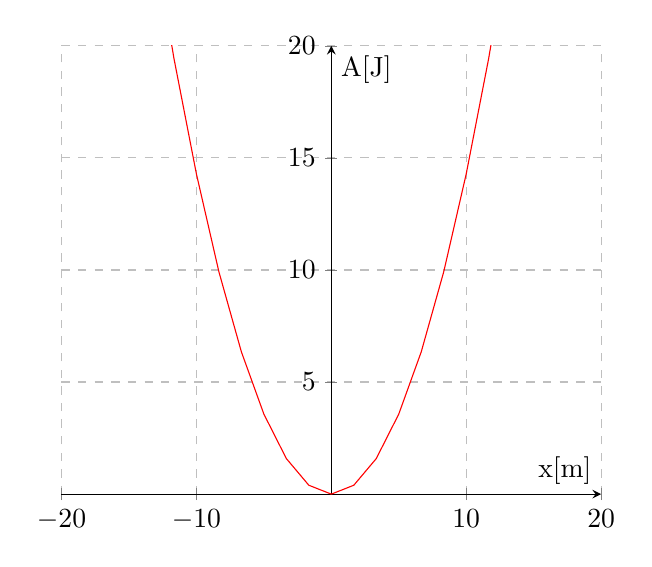
\begin{tikzpicture}
	\begin{axis}[
	    xlabel={x[m]},
	    ylabel={A[J]},
	    xmin=-20, xmax=20,
	    ymin=0, ymax=20,
	    xtick={-20,-10,0,10,20},
	    ytick={0,5,10,15,20},
	    ymajorgrids=true,
	    xmajorgrids=true,
	    grid style=dashed,
	    axis lines=middle,
	]
	 
	\addplot[domain=-20:20,red] {x^2 / 7};

	\end{axis}
\end{tikzpicture}
Tudi ko stiskamo vzmet je delo pozitivno.\\